%%%%%%%%%%%%%%%%%%%%%%%%%%%%%%%%%%%%%%%%%%%%%%%%%%%%%%%%%%%%%%%%%%%%%%%%%%%%%%%%
%2345678901234567890123456789012345678901234567890123456789012345678901234567890
%        1         2         3         4         5         6         7         8
\documentclass[letterpaper, 10 pt, conference]{ieeeconf}  % Comment this line out
                                                          % if you need a4paper
%\documentclass[a4paper, 10pt, conference]{ieeeconf}      % Use this line for a4

\usepackage{float}
                                                          % paper
% uso paquete bookmark para tener bien los outlines.
\usepackage{bookmark}

% Configuro el idioma.
\usepackage[utf8]{inputenc} % Importante para mantener acentos.
\usepackage[spanish, activeacute]{babel} % Requiere: texlive-lang-spanish. Por primera vez hay que ejecutar: texconfig init> log

% Paquete para poder usar acentos en $$.
\usepackage{mathtools}
%\setmathfont{XITS math}

% Para los diagramas de flujo
\usepackage{tikz}
\usetikzlibrary{shapes.geometric, arrows}

% Elementos del diagrama
\tikzstyle{startstop} = [rectangle, rounded corners, 
minimum width=6em, 
minimum height=2em,
text centered, 
draw=black, 
fill=red!30]

\tikzstyle{io} = [trapezium, 
trapezium stretches=true, % A later addition
trapezium left angle=70, 
trapezium right angle=110, 
minimum width=6em, 
minimum height=2em, text centered, 
draw=black, fill=blue!30]

\tikzstyle{block} = [rectangle, 
minimum width=8em, 
minimum height=3em, 
text centered, 
text width=7.5em, 
draw=black, 
fill=white!30]

\tikzstyle{def} = [rectangle, 
minimum width=14em, 
minimum height=3em, 
text centered, 
text width=12em, 
draw=black, 
fill=purple!30]

\tikzstyle{swap_proccess} = [rectangle, 
minimum width=8em, 
minimum height=2em, 
text centered, 
text width=8em, 
draw=black, 
fill=orange!30]

\tikzstyle{process} = [rectangle, 
minimum width=6em, 
minimum height=2em, 
text centered, 
text width=6em, 
draw=black, 
fill=orange!30]

\tikzstyle{decision} = [diamond, 
minimum width=6em, 
minimum height=6em, 
text centered, 
draw=black, 
fill=green!30]
\tikzstyle{arrow} = [thick,->,>=stealth]

\usepackage{siunitx}

% package to get \url
\usepackage{hyperref}
\hypersetup{
  colorlinks=true,
  linkcolor=magenta,
  filecolor=magenta,
  citecolor=magenta,      
  urlcolor=magenta,
}

% Graficos electrónicos
\usepackage[RPvoltages]{circuitikz}

\IEEEoverridecommandlockouts                              % This command is only
                                                          % needed if you want to
                                                          % use the \thanks command
\overrideIEEEmargins
% See the \addtolength command later in the file to balance the column lengths
% on the last page of the document

\usepackage{graphicx}
\usepackage{graphics}

% styling for matlab/octave code.
\usepackage{matlab-prettifier}
% Configuracion, con esto puede agregar ñ.
\lstset{
  literate={ñ}{{\~n}}1
}

\usepackage{listings}

% The following packages can be found on http:\\www.ctan.org
%\usepackage{graphics} % for pdf, bitmapped graphics files
%\usepackage{epsfig} % for postscript graphics files
%\usepackage{mathptmx} % assumes new font selection scheme installed
%\usepackage{times} % assumes new font selection scheme installed
\usepackage{amsmath} % assumes amsmath package installed
%\usepackage{amssymb}  % assumes amsmath package installed

\title{\LARGE \bf Amplificador de audio con boostrapping}

\author{
  Tom\'as Vidal\\
  {\it Circuitos Electróicos II}\\
  {\it Facultad de Ingenier\'ia, UNLP, La Plata, Argentina.}\\
  {\it 30 de Septiembre, 2024.}
}                                            % <-this % stops a space


\begin{document}
\maketitle
\thispagestyle{empty}
\pagestyle{empty}

\section{Placa}
\begin{figure}[H]
  \centering
  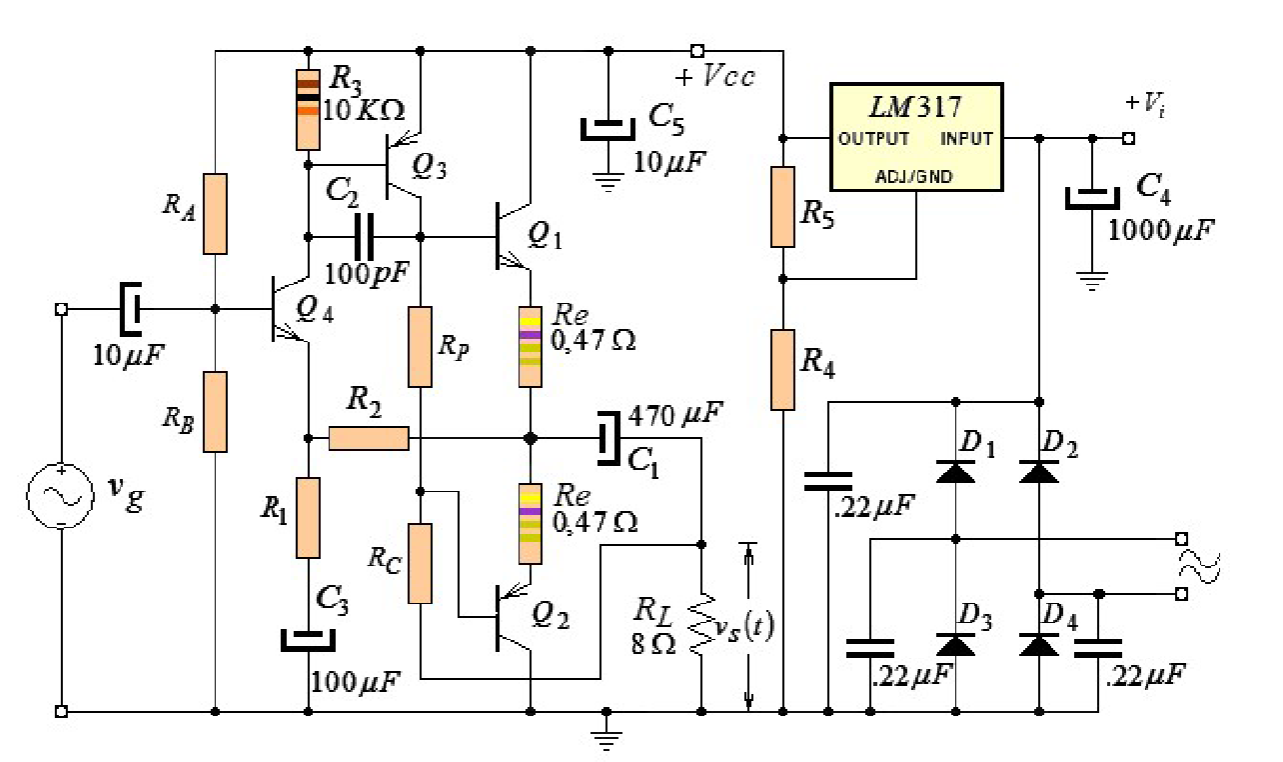
\includegraphics[width=0.43\textwidth]{./imagenes/placa.png}
  \caption{Esquemático de la placa a desarrollar}
  \label{fig:placa}
\end{figure}


\section{Fuente de alimentación}
El diseño se basa en las especificaciones de una alimentación de \textit{entrada} de $220V_{ef}$ con un \textit{ripple} del $10\%$; y una \textit{salida} en el regulador de 13V con una variación del $7.7\%$ \\
\hspace{10em} Para cumplir estas especificaciones se emplearon las curvas de \textbf{Schade} que permiten obtener que tensión sin regular se necesita en el capcitor de filtarado, y la tensión alterna que debe haber en el secundario para satisfacer estas especificaciones.
\begin{figure}[H]
  \centering
  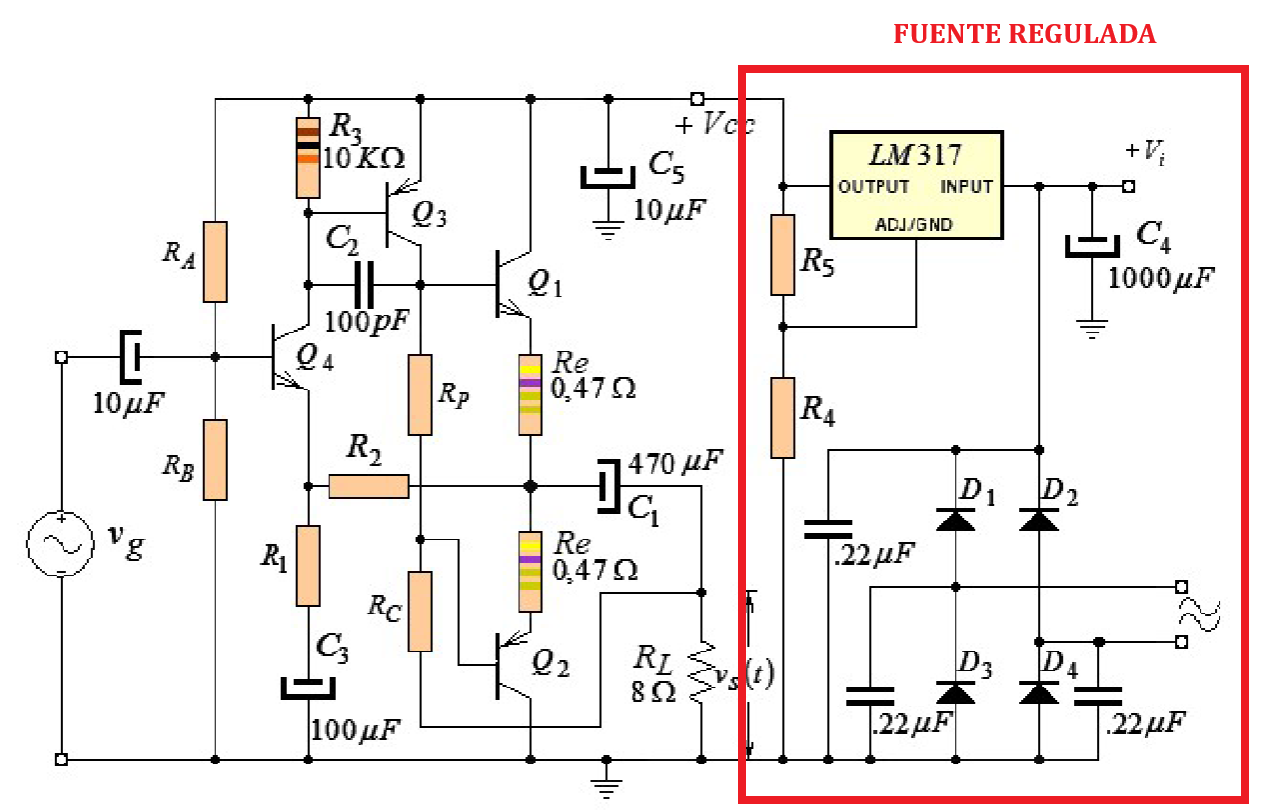
\includegraphics[width=0.43\textwidth]{./imagenes/placa_fuente.png}
  \caption{Sección de la fuente regulada}
  \label{fig:placa_fuente}
\end{figure}

Se parte de que en el secundario del transformador se tendrá un \textit{ripple} del $10\%$, así como en el primario. Entonces para el peor caso, \textit{es decir cuando el secundario tiene el pico de tensión mínimo}, se calcula por \textbf{Schade} el valor


\end{document}